\documentclass[8pt,a4paper,compress]{beamer}

\usepackage{/home/siyer/lib/slides}

\usepackage{fancyvrb}

\newcommand{\mm}[1]{$#1$}
\newcommand{\derives}{\stackrel{*}{\Rightarrow}}
\newcommand{\expo}[2]{$#1^{#2}$}
\newcommand{\subs}[2]{${#1}_{#2}$}

\DefineVerbatimEnvironment
{production}{Verbatim}
{fontfamily=timesroman,commandchars=\\\{\}}
\newenvironment{spaced}
{
\smallskip
\hspace{.5cm}
\begin{minipage}[c]{\textwidth}
}
{
\end{minipage}
\smallskip
}

\title{Register Allocation}
\date{}

\begin{document}
\begin{frame}
\vfill
\titlepage
\end{frame}

\begin{frame}
\frametitle{Outline}
\tableofcontents
\end{frame}

\section{Introduction}
\begin{frame}[fragile]
\pause

Register allocation is the process of assigning as many local variables and temporaries to physical registers as possible

\pause
\bigskip

The more values that we can keep in registers instead of memory, the faster our programs will run

\pause
\bigskip

With respect to our LIR, we wish to assign physical registers to each of the virtual registers that serve as operands to instructions

\pause
\bigskip

But there are often fewer physical registers than there are virtual registers

\pause
\bigskip

Sometimes, as program execution progresses, some values in physical registers will have to be spilled to memory while the register is used for another purpose, and then reloaded when those values are needed again

\pause
\bigskip

Code must be generated for storing spilled values and then for reloading those values at appropriate places; we would like to minimize this spilling (and reloading) of values to and from memory
\end{frame}

\begin{frame}[fragile]
\pause

Any register allocation strategy must determine how to most effectively allocate physical registers to virtual registers and, when spilling is necessary, which physical registers to spill to make room for assignment to other virtual registers

\pause
\bigskip

The problem of register allocation is NP-complete in general

\pause
\bigskip

Register allocation that focuses on just a single basic block, or even just a single statement,
is said to be local

\pause
\bigskip

Register allocation that considers the entire flow graph of a method is said to be global

\pause
\bigskip

We will look at a nai\"{i}ve (local) strategy as well as a global strategy based on graph coloring
\end{frame}

\section{Na\"{i}ve Register Allocation}
\begin{frame}[fragile]
\pause

The na\"{i}ve register allocation strategy simply sequences through the operations in the (LIR) code, assigning physical registers to virtual registers

\pause
\bigskip

Once all physical registers have been assigned, and if there are additional virtual registers to deal with, we begin spilling physical registers to memory

\pause
\bigskip

There is no strategy for determining which registers to spill; for example, one might simply sequence through the physical registers a second time in the same order they were assigned the first time, spilling each to memory as it is re-needed

\pause
\bigskip

When a spilled value used again, it must be reloaded into a (possibly different) register

\pause
\bigskip

Such a strategy works just fine when there are as many physical registers as there are virtual registers; in fact, it is as effective as any other register allocation scheme in this case

\pause
\bigskip

When there are many more virtual registers than physical registers, which is always the case, performance of the na\"{i}ve strategy degrades rapidly as physical register values must be repeatedly spilled and reloaded
\end{frame}

\begin{frame}[fragile]
\pause

Following is the SPIM code generated by \jmm using the na\"{i}ve register allocation strategy (and just three physical registers \$t0, \$t1, and \$t2) for \lstinline{Factorial.computeIter()} method

\begin{lstlisting}[language={}]
    subu    $sp,$sp,48 	 # Stack frame is 48 bytes long
    sw      $ra,44($sp) 	 # Save return address
    sw      $fp,40($sp) 	 # Save frame pointer
    sw      $t0,36($sp) 	 # Save register $t0
    sw      $t1,32($sp) 	 # Save register $t1
    sw      $t2,28($sp) 	 # Save register $t2
    addiu   $fp,$sp,44 	 # Save frame pointer

Factorial.computeIter.0:

Factorial.computeIter.1:
    li $t0,1
    sw $t0,0($sp)
    move $t1,$a0
    sw $t1,8($sp)
    lw $t0,0($sp)
    move $t2,$t0
    sw $t2,16($sp)

Factorial.computeIter.2:
    li $t0,0
    sw $t0,4($sp)
    lw $t1,8($sp)
    lw $t0,4($sp)
    ble $t1,$t0,Factorial.computeIter.4
    j Factorial.computeIter.3

\end{lstlisting}
\end{frame}

\begin{frame}[fragile]
\pause

\begin{lstlisting}[language={}]
Factorial.computeIter.3:
    li $t1,-1
    sw $t1,12($sp)
    lw $t1,8($sp)
    lw $t1,12($sp)
    add $t2,$t1,$t1
    sw $t2,20($sp)
    lw $t2,16($sp)
    lw $t1,8($sp)
    mul $t0,$t2,$t1
    sw $t0,24($sp)
    lw $t0,24($sp)
    move $t2,$t0
    sw $t2,16($sp)
    lw $t2,20($sp)
    move $t1,$t2
    sw $t1,8($sp)
    j Factorial.computeIter.2

Factorial.computeIter.4:
    lw $t2,16($sp)
    move $v0,$t2
    j Factorial.computeIter.restore

Factorial.computeIter.restore:
    lw      $ra,44($sp) 	 # Restore return address
    lw      $fp,40($sp) 	 # Restore frame pointer
    lw      $t0,36($sp) 	 # Restore register $t0
    lw      $t1,32($sp) 	 # Restore register $t1
    lw      $t2,28($sp) 	 # Restore register $t2
    addiu   $sp,$sp,48 	 # Pop stack
    jr      $ra 	 # Return to caller
\end{lstlisting}
\end{frame}

\section{Register Allocation by Graph Coloring}
\begin{frame}[fragile]
\pause

Global register allocation works with a method's entire control-flow graph to map virtual registers to physical registers

\pause
\bigskip

One wants to minimize spills to memory; where spills are necessary, one wants to avoid using them within deeply nested loops

\pause
\bigskip

The basic tool in global register allocation is the liveness interval, the sequence of instructions for which a virtual register holds a meaningful value

\pause
\bigskip

A liveness interval for a virtual register extends from the first instruction that assigns it a value to the last instruction that uses its value

\pause
\bigskip

A more accurate liveness interval has ``holes'' in the sequence, where a virtual register does not contain a useful value; for example, a hole occurs from where the previously assigned value
was last used (or read) to the next assignment (or write) of a new value
\end{frame}

\begin{frame}[fragile]
\pause

Consider the control-flow graph for \lstinline{Factorial.computeIter()}
\begin{center}
\visible<2->{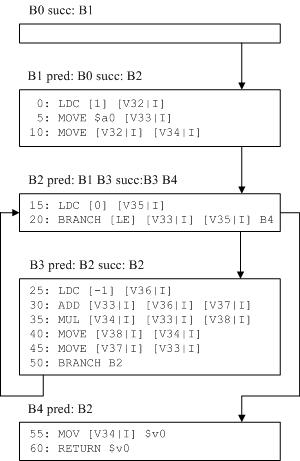
\includegraphics[scale=0.6]{{figures/figure07.01}.jpg}}
\end{center}
\end{frame}

\begin{frame}[fragile]
\pause

The liveness intervals for the above code are illustrated in the following figure
\begin{center}
\visible<2->{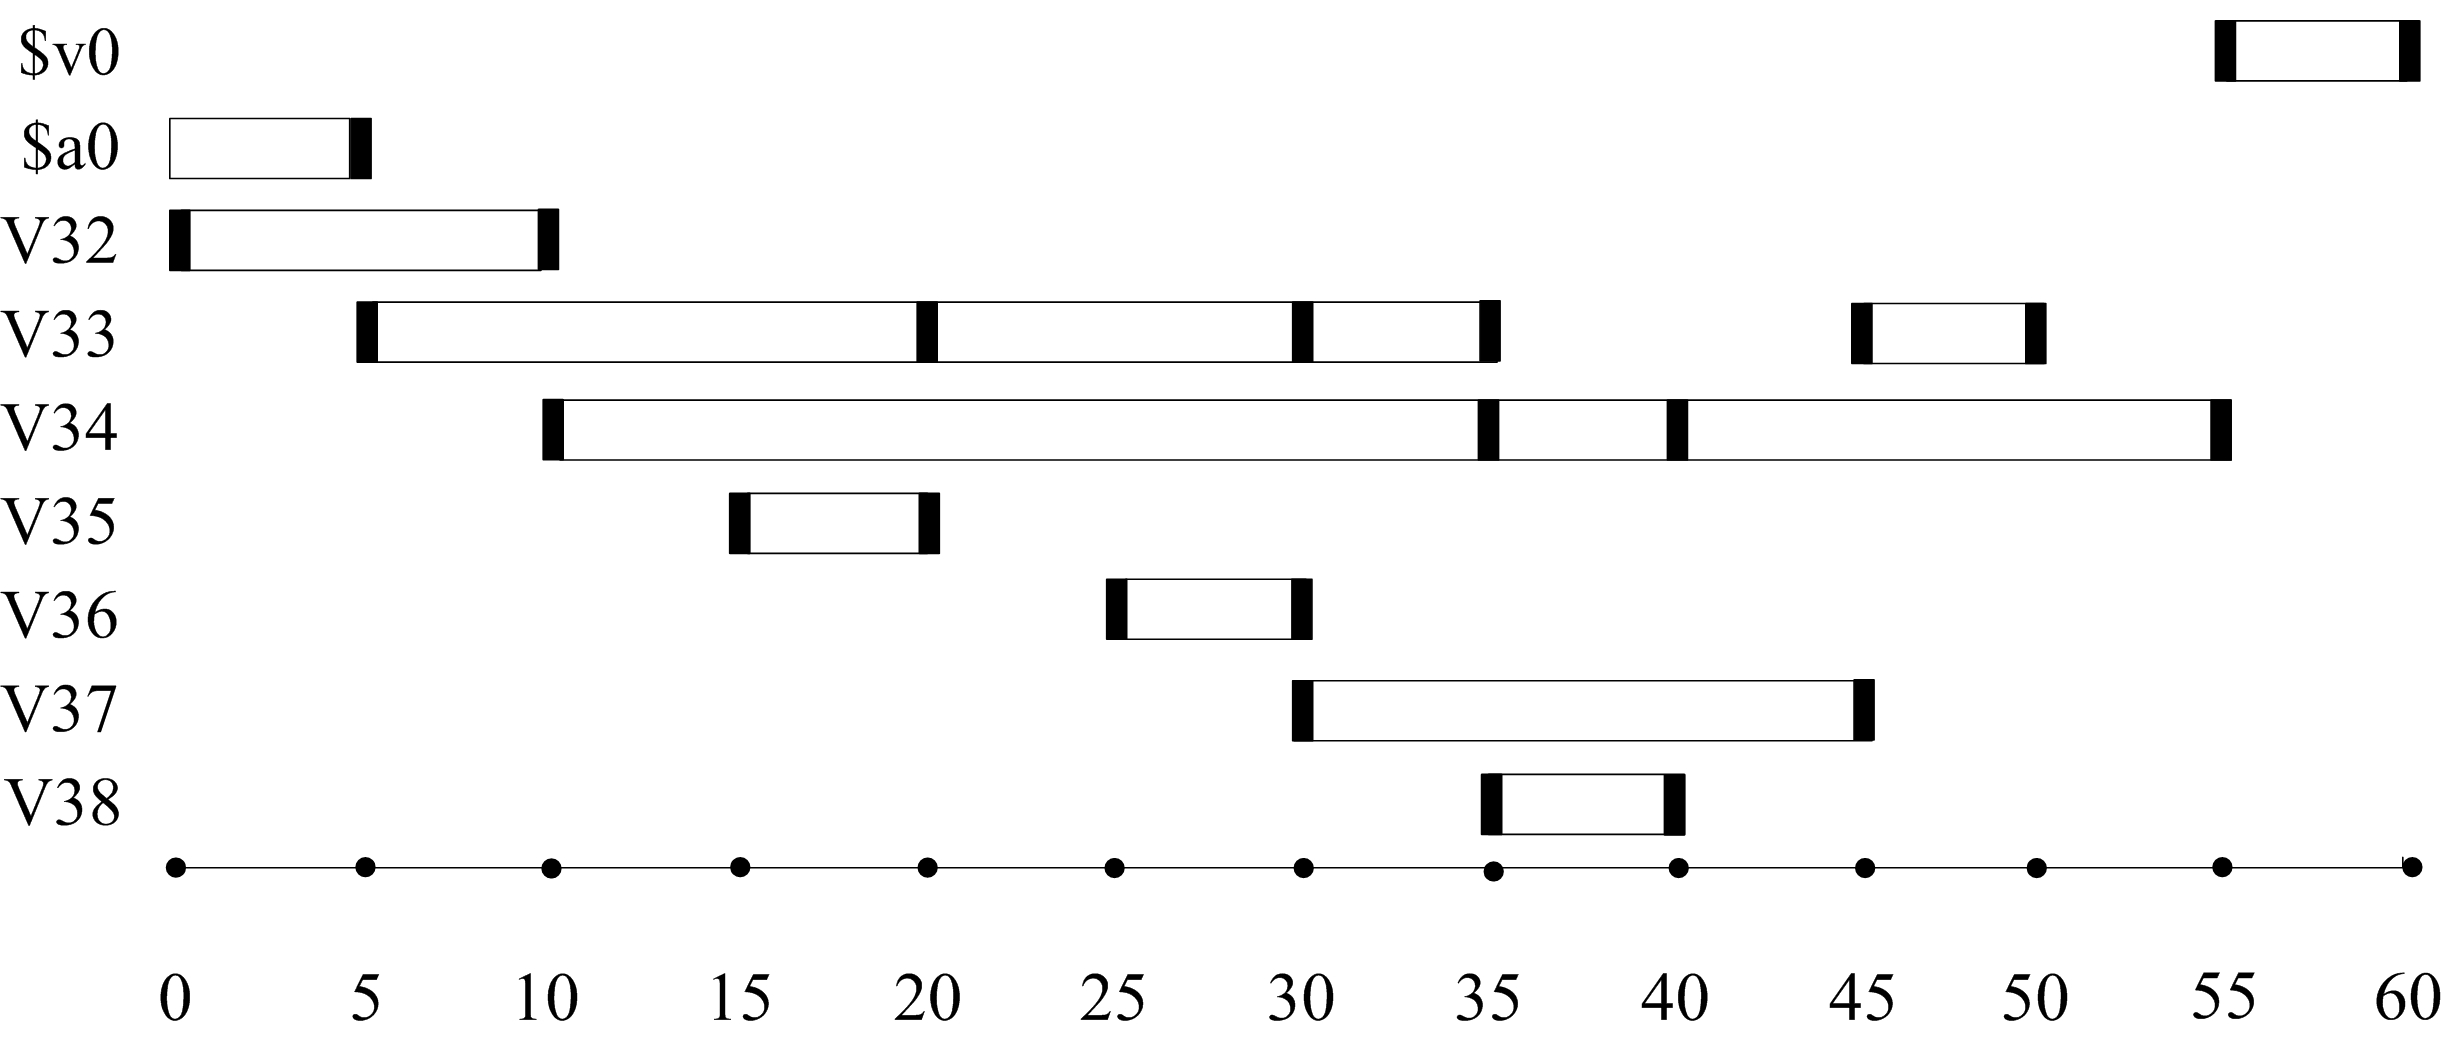
\includegraphics[scale=0.6]{{figures/figure07.02}.jpg}}
\end{center}

\bigskip

The numbers on the horizontal axis represent instruction ids and the vertical axis is labeled with register IDs

\bigskip

The darker vertical segments in the intervals identify use positions: a use position is a position in the interval where either the register is defined (ie, written) or the register is being used (ie, read)
\end{frame}

\begin{frame}[fragile]
\pause

We first compute, for each block, two local liveness sets: liveUse and liveDef

\pause
\bigskip

LiveUse operands are those operands that are read (or used) before they are written (defined) in the block's instruction sequence

\pause
\bigskip

LiveDef operands are those operands that are written to (defined) by some instruction in the block

\pause

\begin{algorithm}[H]
\begin{algorithmic}
\REQUIRE The control-flow graph $g$ for a method
\ENSURE Two sets for each basic block: liveUse, registers used before they are overwritten (defined) in the block and liveDef, registers that are defined in the block
\FOR {block $b$ in $g$.blocks}
\STATE Set $b$.liveUse $ \gets \{\}$
\STATE Set $b$.liveDef $ \gets \{\}$
\FOR {instruction $i$ in $b$.instructions}
\FOR {virtual register $v$ in $i$.readOperands}
\IF {$v \notin b$.liveDef}
\STATE $b$.liveUse.add($v$) 
\ENDIF
\ENDFOR
\FOR {virtual register $v$ in $i$.writeOperands}
\STATE $b$.liveDef.add($v$)
\ENDFOR
\ENDFOR
\ENDFOR
\end{algorithmic}
\caption{Computing Local Liveness Information}
\end{algorithm}
\end{frame}

\begin{frame}[fragile]
\pause

The control-flow graph for \lstinline{Factorial.computeIter()} with its local liveness sets computed is illustrated below
\begin{center}
\visible<2->{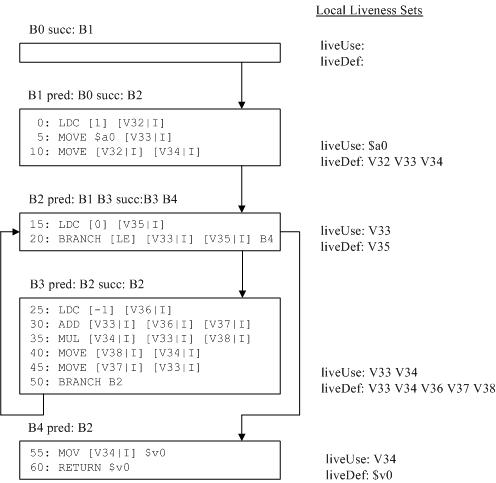
\includegraphics[scale=0.6]{{figures/figure07.03}.jpg}}
\end{center}
\end{frame}

\begin{frame}[fragile]
\pause

We can compute the set of operands that are live at the beginning and end of a block
using a backward data-flow analysis

\pause
\bigskip

We call the set of operands that are live at the start of a block liveIn

\pause
\bigskip

We call the set of operands that are live at the end of a block liveOut

\pause

\begin{algorithm}[H]
\begin{algorithmic}
\REQUIRE The control-flow graph $g$ for a method, and the local liveness sets liveUse and liveDef for every basic block
\ENSURE Two sets for each basic block: liveIn, registers live at the beginning of the block, and liveOut, registers that are live at the end of the block
\REPEAT
    \FOR {block $b$ in $g$.blocks in reverse order}
        \STATE $b$.liveOut $ \gets \{\} $
        \FOR {block $s$ in $b$.successors}
            \STATE $b$.liveOut $\gets$ $b$.liveOut $\cup$ $s$.liveIn
        \ENDFOR
        \STATE $b$.liveIn $\gets$  ($b$.liveOut $-$  $b$.liveDef) $\cup$  $b$.liveUse
    \ENDFOR
\UNTIL{ no liveOut has changed }

\end{algorithmic}
\caption{Computing Global Liveness Information}
\end{algorithm}
\end{frame}

\begin{frame}[fragile]
\pause

The computation of the global liveness information for \lstinline{Factorial.computeIter()} requires three iterations

\pause
\bigskip

After first iteration
\begin{lstlisting}[language={}]
B4 liveIn:  V34
B4 liveOut:
B3 liveIn:  V33 V34
B3 liveOut:
B2 liveIn:  V33 V34
B2 liveOut: V33 V34
B1 liveIn:  $a0                                                                 
B1 liveOut: V33 V34                                                             
B0 liveIn:  $a0
B0 liveOut: $a0
\end{lstlisting}

\pause

After second iteration
\begin{lstlisting}[language={}]
B4 liveIn:  V34
B4 liveOut:
B3 liveIn:  V33 V34
B3 liveOut: V33 V34
B2 liveIn:  V33 V34
B2 liveOut: V33 V34
B1 liveIn:  $a0                                                                 
B1 liveOut: V33 V34                                                             
B0 liveIn:  $a0
B0 liveOut: $a0
\end{lstlisting}
\end{frame}

\begin{frame}[fragile]
\pause

After third (and final) iteration
\begin{lstlisting}[language={}]
B4 liveIn:  V34
B4 liveOut:
B3 liveIn:  V33 V34
B3 liveOut: V33 V34
B2 liveIn:  V33 V34
B2 liveOut: V33 V34
B1 liveIn:  $a0
B1 liveOut: V33 V34
B0 liveIn:  $a0                                                                 
B0 liveOut: $a0
\end{lstlisting}

\pause
\bigskip

To build the intervals, we make a single pass over the blocks and instructions, again in reverse order
\end{frame}

\begin{frame}[fragile]
\pause

\begin{algorithm}[H]
\begin{algorithmic}
\REQUIRE The control-flow graph $g$ for a method with LIR, and the liveIn and liveOut sets for each basic block
\ENSURE A liveness interval for each register, with ranges and use positions
\FOR {block $b$ in $g$.blocks in reverse order}
    \STATE int $blockFrom$ $\gets$ $b$.firstInstruction.id
    \STATE Set $blockTo$ $\gets$ $b$.lastInstruction.id
    \FOR {register $r$ in $b$.liveOut}
        \STATE intervals[$r$].addOrExtendRange($blockFrom$, $blockRange$)
    \ENDFOR
    \FOR { instruction $i$ in $b$.instructions in reverse order}
        \IF {$i$.isAMethodCall}
            \FOR {physical register $r$ in the set of physical registers}
                \STATE intervals[$r$].addRange($i$.id, $i$.id)
            \ENDFOR
        \ENDIF
        \FOR {virtual register $r$ in $i$.writeOperands}
            \STATE intervals[$r$].firstRange.from $\gets$ $i$.id
            \STATE intervals[$r$].addUsePos($i$.id)
        \ENDFOR
        \FOR {virtual register $r$ in $i$.readOperands}
            \STATE intervals[$r$].addOrExtendRange($blockFrom$, $i$.id)
            \STATE intervals[$r$].addUsePos($i$.id)
        \ENDFOR
    \ENDFOR
\ENDFOR
\end{algorithmic}
\caption{Building Liveness Intervals}
\end{algorithm}
\end{frame}

\begin{frame}[fragile]
\pause

We first add ranges for all registers that are in liveOut, extending from the start of the block to the end

\pause
\bigskip

As we iterate through the instructions of each block, in reverse order, we add or modify ranges
\begin{itemize}
\item When we encounter a subroutine call, we add ranges of length one at the call's position to the intervals of all physical registers, because we assume the subroutine itself will use these registers and so we want to force spills

\item If the instruction has a register that is written to, then we adjust the first (most recent) range's start position to be the position of the (writing) instruction, and we record the use position

\item For each register that is read (or used) in the instruction, we add a new range extending to this instruction's position; initially, the new range begins at the start of the block, and a write may cause the start position to be re-adjusted --- note that \lstinline{addOrExtendRange()} operation merges contiguous ranges into one
\end{itemize}
\end{frame}

\begin{frame}[fragile]
\pause

Consider the basic block \lstinline{B3} of the LIR for \lstinline{Factorial.computeIter()}
\begin{lstlisting}[language={}]
B3
25: LDC [-1] [V36|I]
30: ADD [V33|I] [V36|I] [V37|I]
35: MUL [V34|I] [V33|I] [V38|I]
40: MOVE [V38|I] [V34|I]
45: MOVE [V37|I] [V33|I]
50: BRANCH B2
\end{lstlisting}

The progress of building intervals for the basic block is illustrated below
\begin{center}
\visible<2->{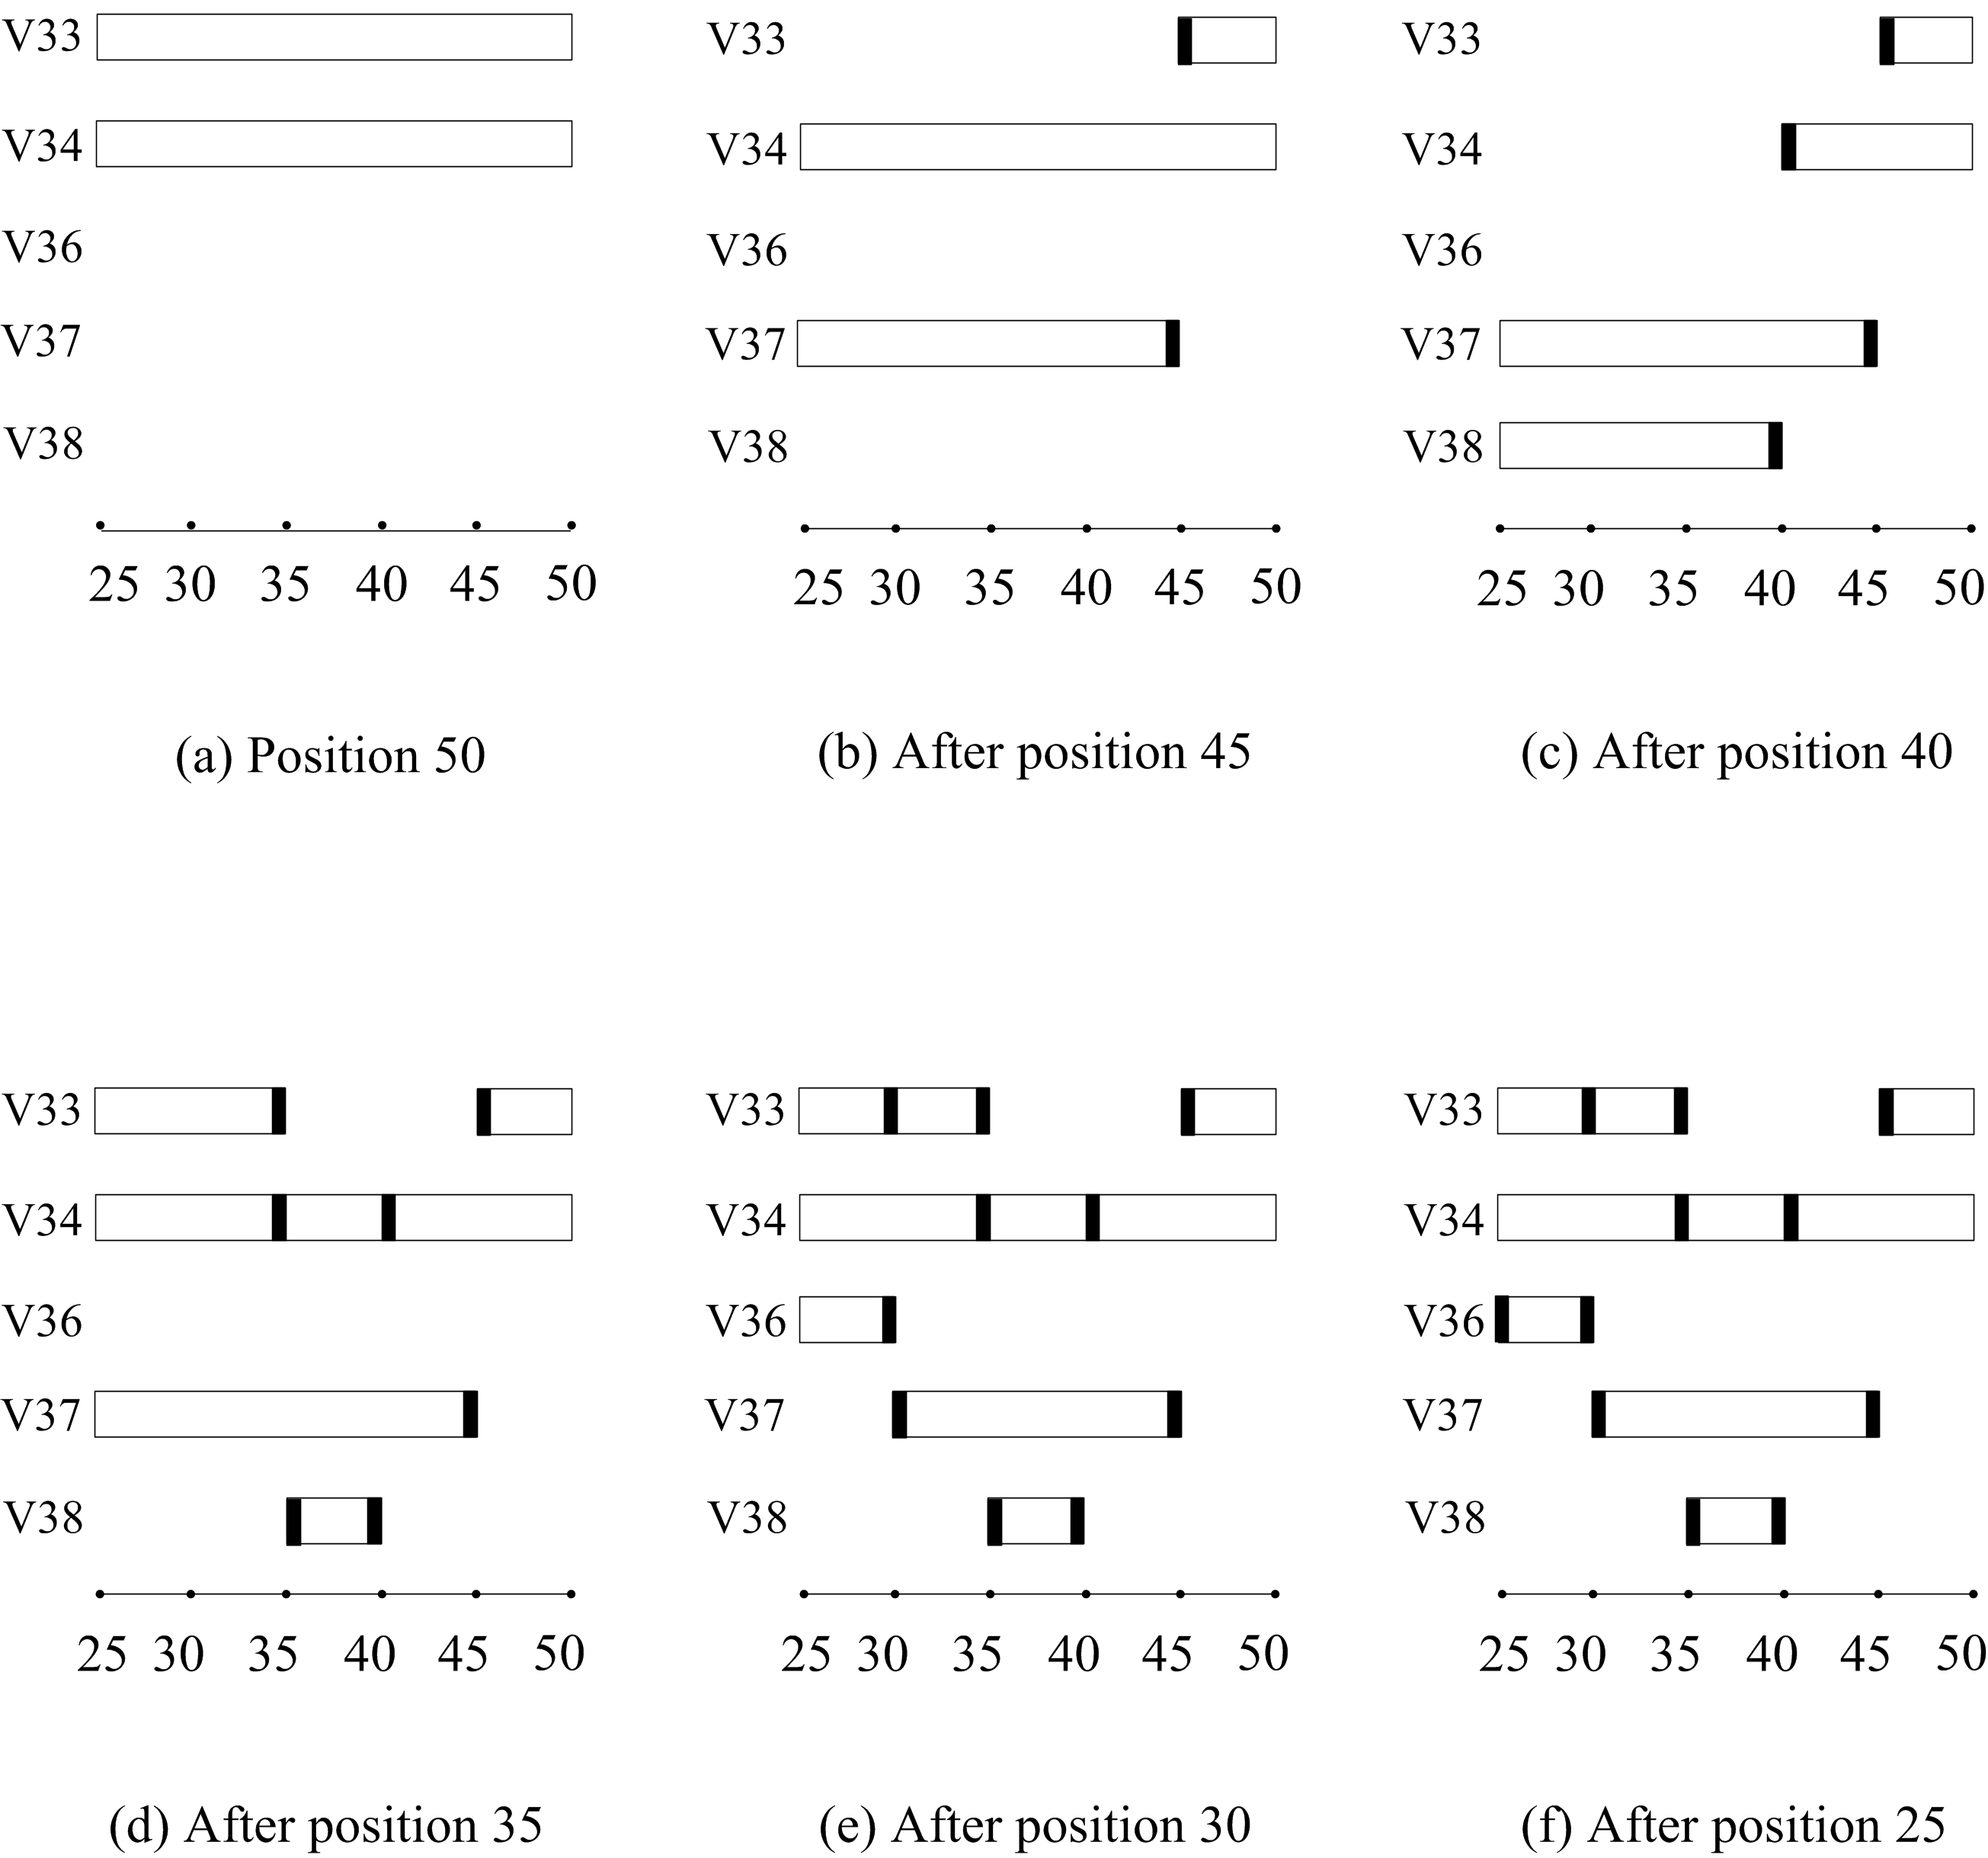
\includegraphics[scale=0.39]{{figures/figure07.04}.jpg}}
\end{center}
\end{frame}

\begin{frame}[fragile]
\pause

In graph coloring register allocation, we start with an interference graph built from the
liveness intervals

\pause
\bigskip

An interference graph consists of a set of nodes, one for each virtual register or liveness interval, and a set of edges

\pause
\bigskip

There is an edge between two nodes if the corresponding intervals interfere, ie, if they are live at the same time

\pause
\bigskip

For example, reconsider the liveness intervals for the virtual registers \$V32 -- \$V38 of \lstinline{Factorial.computeIter()}

\begin{center}
\visible<5->{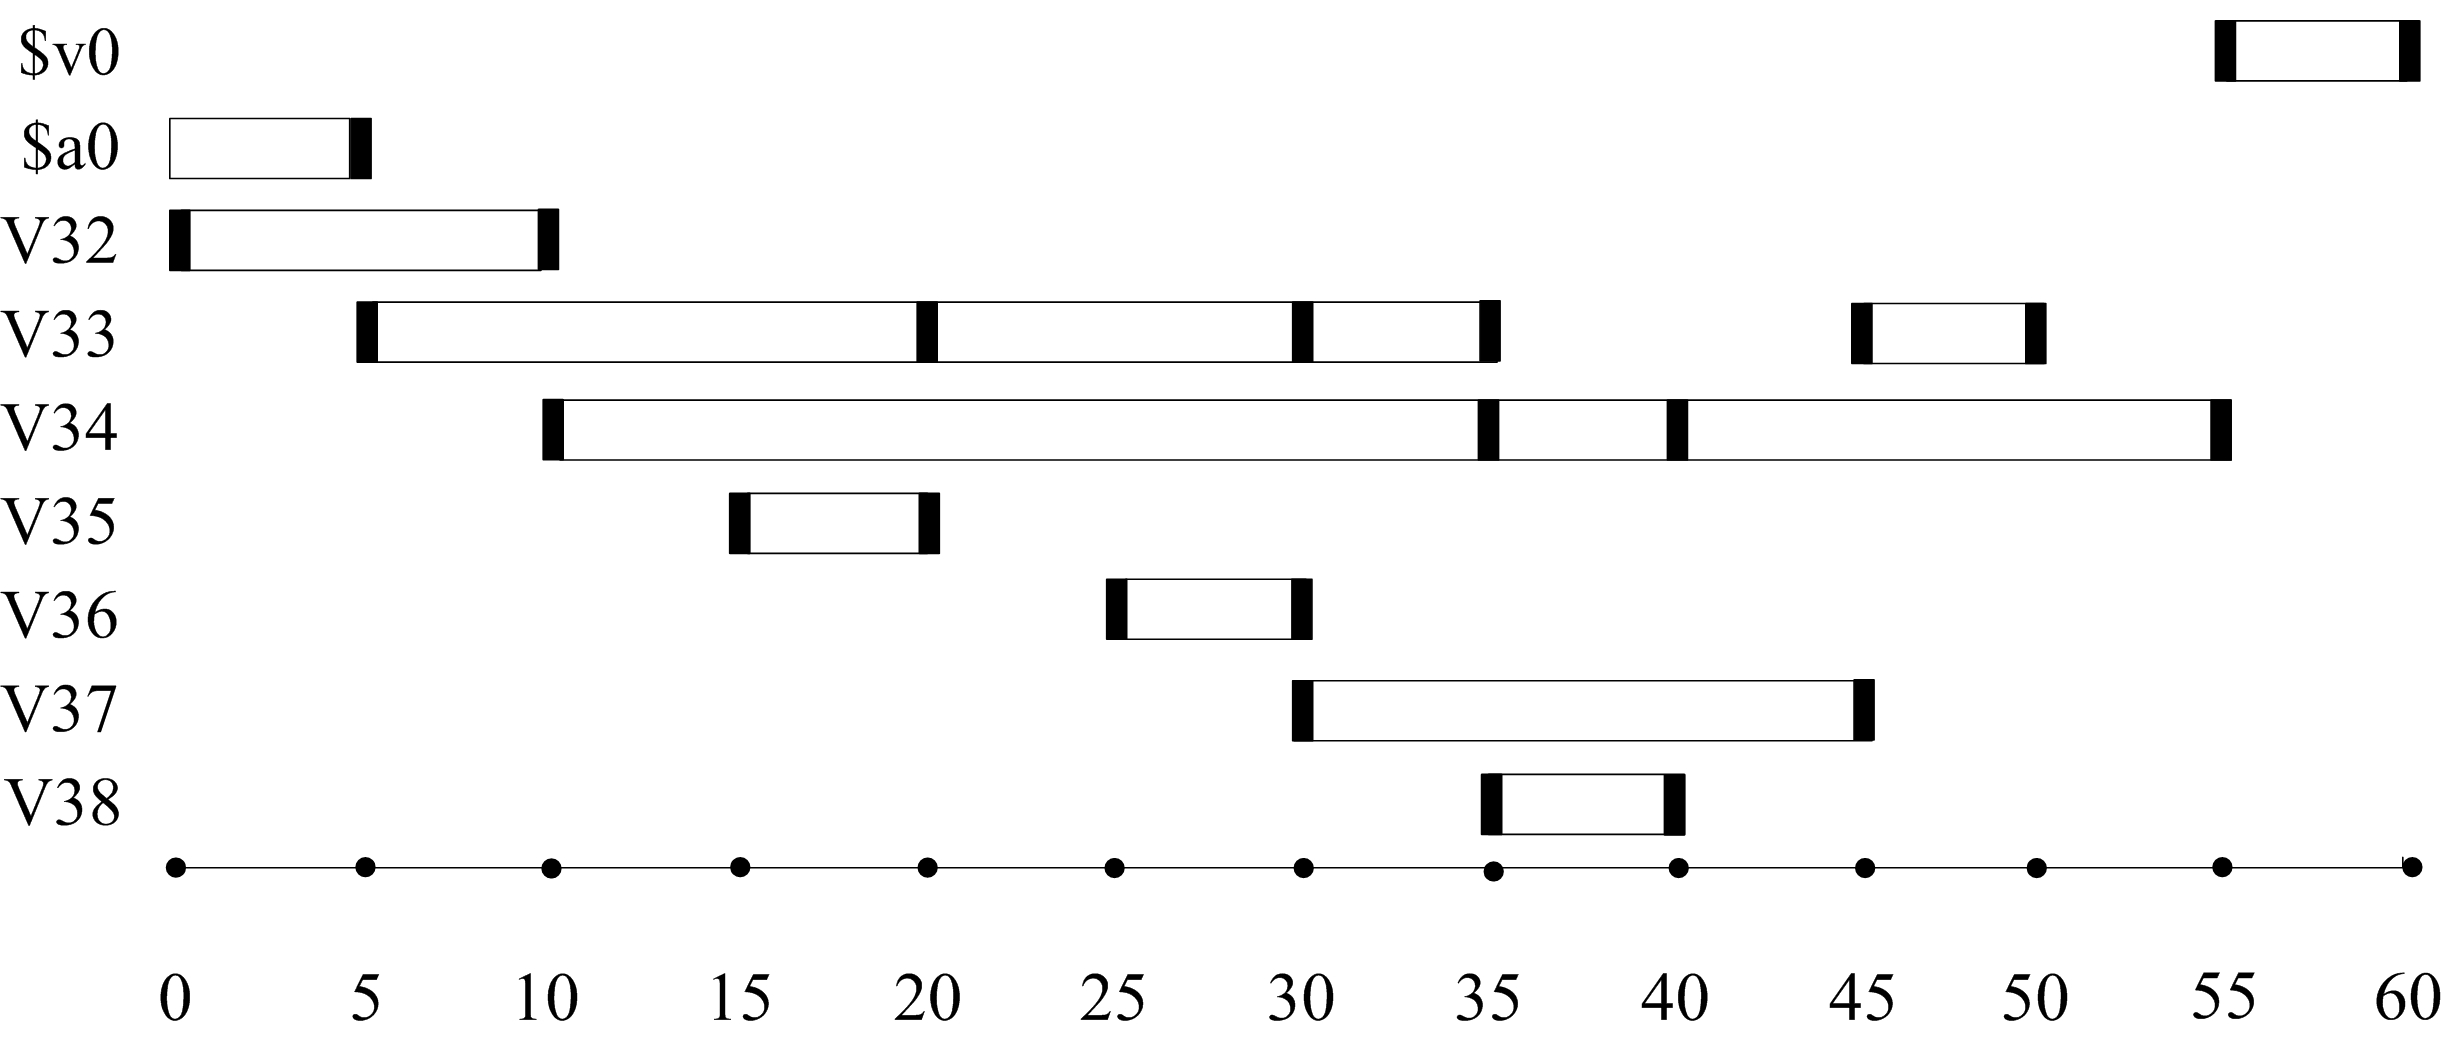
\includegraphics[scale=0.6]{{figures/figure07.02}.jpg}}
\end{center}
\end{frame}

\begin{frame}[fragile]
\pause

The interference graph for \lstinline{Factorial.computeIter()} is shown below
\begin{center}
\visible<2->{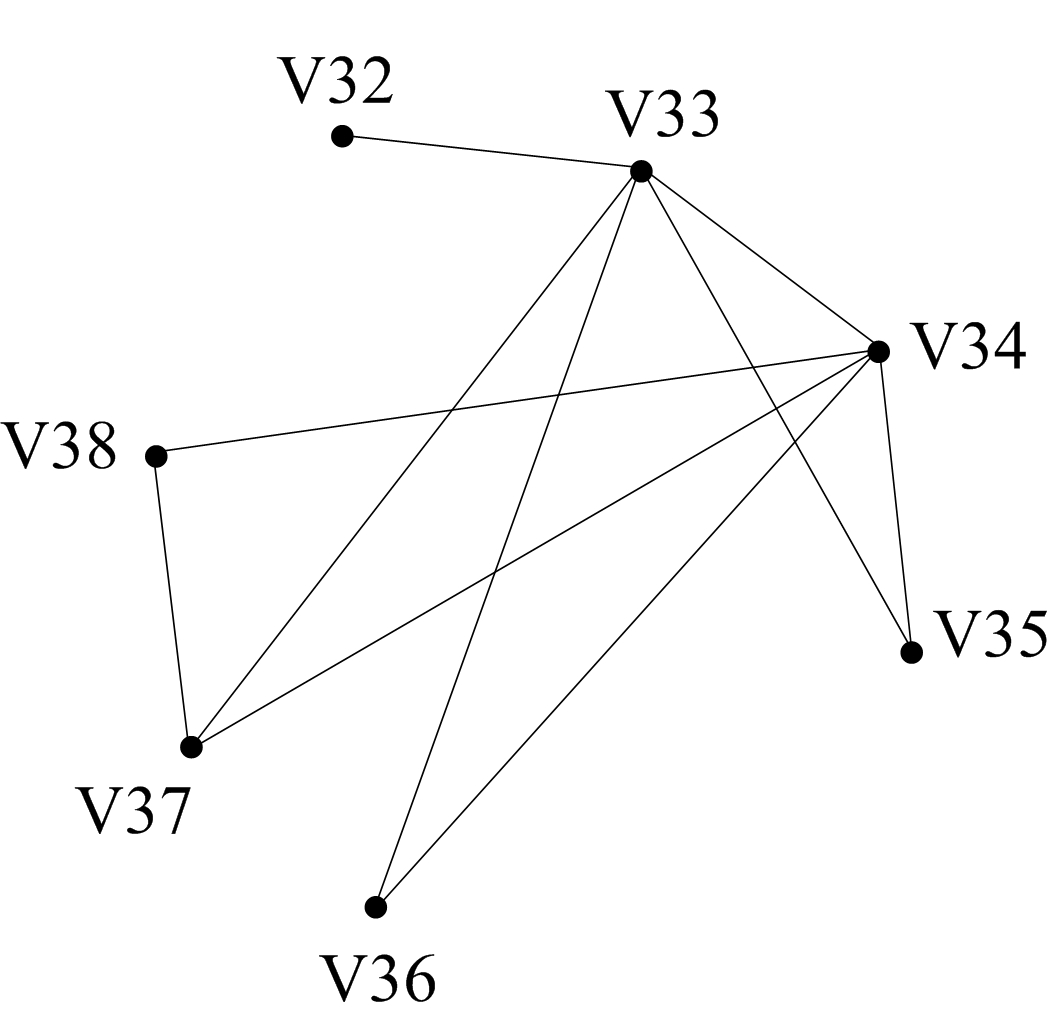
\includegraphics[scale=0.6]{{figures/figure07.08}.jpg}}
\end{center}

\pause
\bigskip

We say that a graph has an $R$-coloring if it can be colored using $R$ distinct colors, or in our case $R$ distinct physical registers

\pause
\bigskip

To exhaustively find such an $R$-coloring for $R \ge 2$ has long been known to be NP-complete

\pause
\bigskip

But there are two heuristics available to us for simplifying the graph
\end{frame}

\begin{frame}[fragile]
\pause

\begin{enumerate}
\item Degree $< R$ heuristic: a graph with a node of degree $< R$ is $R$-colorable if and only if the graph with that node removed is $R$-colorable; we may use this rule to prune the graph, removing one node of degree $< R$ at a time and pushing it onto a stack; we continue removing nodes until either all nodes have been pruned or until we reach a state where all remaining nodes have degrees $\ge R$

\item Optimistic heuristic: we use a function \lstinline{spillCost()} to find a node having the smallest cost of spilling its associated virtual register; we mark that register for possible spilling and remove the node (and its edges) and push it onto the stack in the hope that we will not really have to spill it later
\end{enumerate}
\end{frame}

\begin{frame}[fragile]
\pause

Pruning of the above interference graph with $R = 3$ is shown below
\begin{center}
\visible<2->{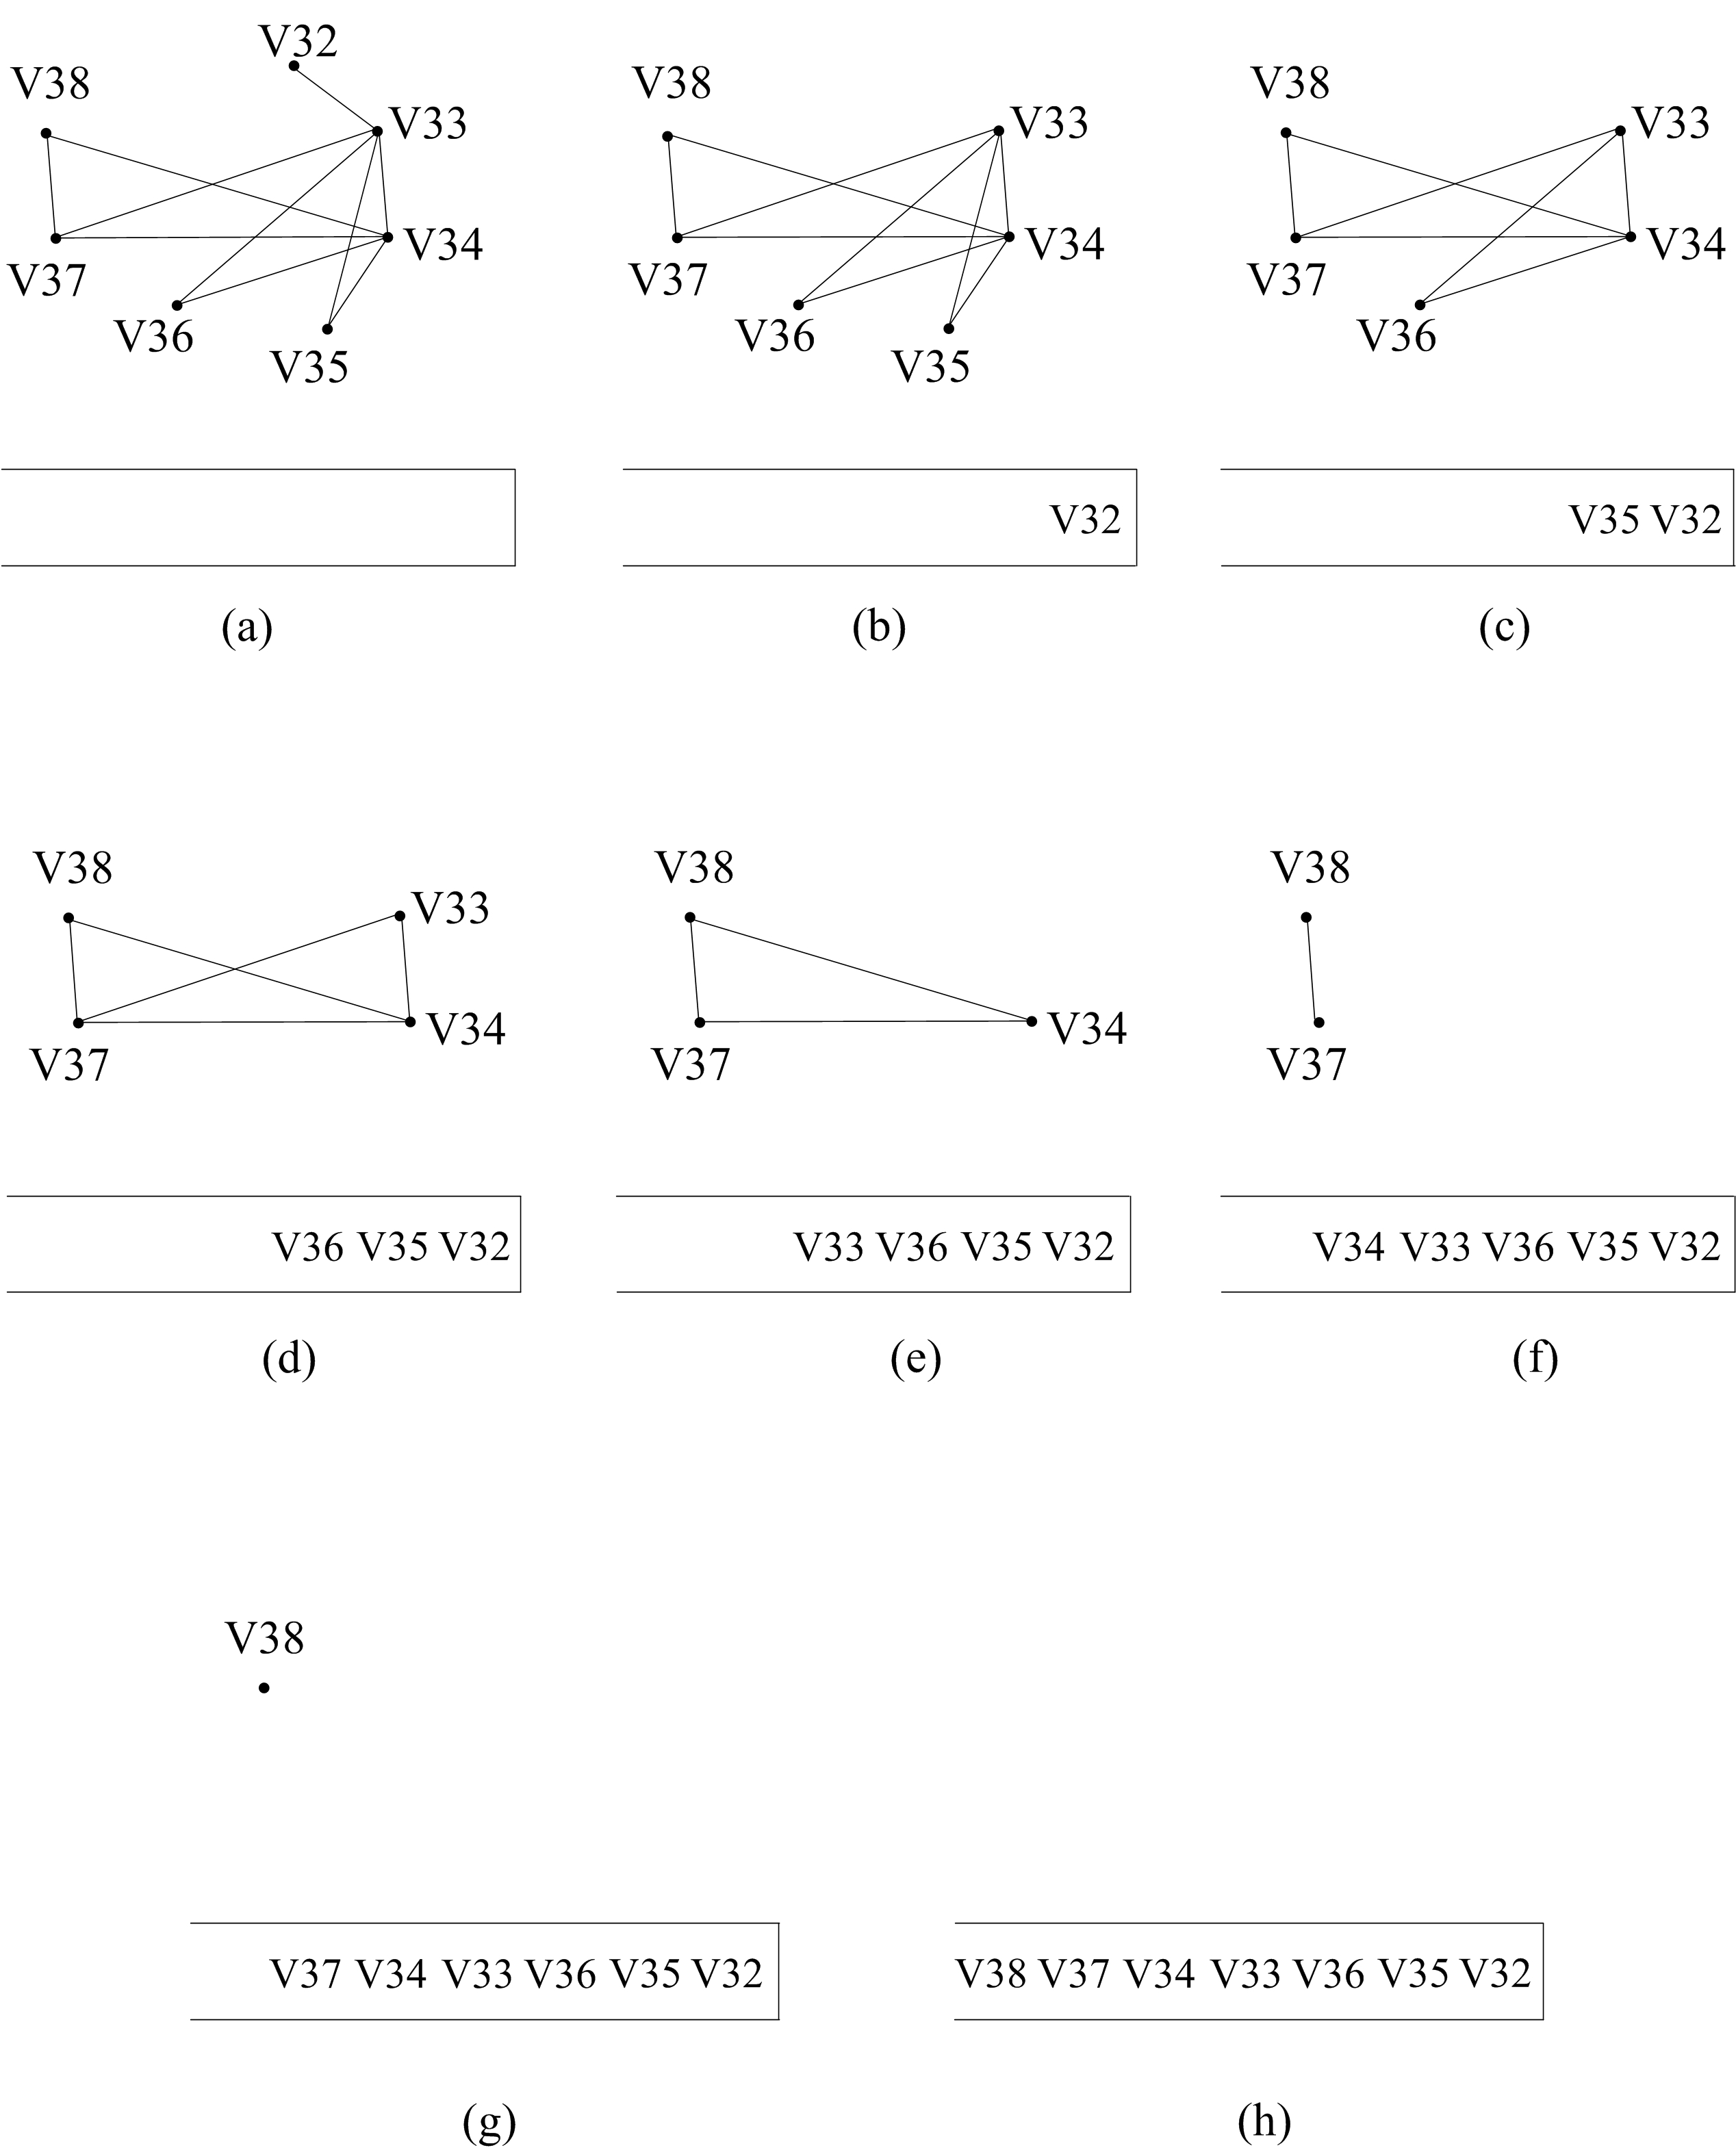
\includegraphics[scale=0.5]{{figures/figure07.09}.jpg}}
\end{center}
\end{frame}

\begin{frame}[fragile]
\pause

We may then pop the virtual registers off of the list, one at a time, and try to assign physical register numbers ($r1$, $r2$, or $r3$) to each in such a way that adjacent virtual registers are never assigned the same physical register

\pause
\bigskip

A possible assignment is
\begin{production}
    V38 r1
    V37 r2
    V34 r3
    V33 r1
    V36 r2
    V35 r2
    V32 r2
\end{production}

\pause

Imposing this mapping onto our LIR for \lstinline{Factorial.computeIter()} gives us
\begin{lstlisting}[language={}]
  B0

  B1
  0: LDC [1] r2
  5: MOVE $a0 r1
  10: MOVE r2 r3

\end{lstlisting}
\end{frame}

\begin{frame}[fragile]
\pause

\begin{lstlisting}[language={}]
  B2
  15: LDC [0] r2
  20: BRANCH [LE] r1 r2 B4

  B3
  25: LDC [-1] r2
  30: ADD r1 r2 r2
  35: MUL r3 r1 r1
  40: MOVE r1 r3
  45: MOVE r2 r1
  50: BRANCH B2

  B4
  55: MOVE r3 $v0                                                               
  60: RETURN $v0
\end{lstlisting}
\end{frame}

\begin{frame}[fragile]
\pause

\begin{algorithm}[H]
\begin{algorithmic}
\REQUIRE The control-flow graph $g$ for a method with LIR that makes use of virtual registers
\ENSURE The same $g$ but with virtual registers replaced by physical registers
\STATE $registersAssignedSuccessfully$ $\gets$ \lstinline{false}
\REPEAT
    \REPEAT
        \STATE buildIntervals()
        \STATE buildInterferenceGraph()
    \UNTIL {\NOT coalesceRegistersSuccessful()}
        \STATE buildAdjacencyLists()
        \STATE computeSpillCosts()
	\STATE pruneGraph()
        \STATE $registersAssignedSuccessfully$ $\gets$ assignRegisters()

        \IF {\NOT $registersAssignedSuccessfully$}
            \STATE generateSpillCode()
        \ENDIF
\UNTIL {$registersAssignedSuccessfully$}
\end{algorithmic}
\caption{Graph Coloring Register Allocation}
\end{algorithm}
\end{frame}

\begin{frame}[fragile]
\pause

Coalescing registers reduces both the number of virtual registers and the number of moves

\pause
\bigskip

The method \lstinline{coalesceRegistersSuccessful()} returns \lstinline{true} if it is able to coalesce two registers and \lstinline{false} otherwise; this boolean result is used to insure that any register coalescing is followed by a rebuilding of the intervals and the interference graph

\pause
\bigskip

We use both an adjacency matrix and an adjacency list representation for the interference graph

\pause
\bigskip

During the pruning process we may reach a state where only nodes with degree $\ge R$ remain in the graph, in which case, our algorithm must choose a node with the smallest spill cost

\pause
\bigskip

The spill cost of a register depends on the loop depths of the positions where the register must be stored to or loaded from memory

\pause
\bigskip

An option is summing up the uses and definitions, using a factor of $10^\text{depth}$ for taking loop depth into account; it's better to re-compute the value for a register when it is cheaper than spilling
and reloading that same value
\end{frame}
\end{document}
